\section{Design}

\subsection{Design Overview}
\label{sec:DesignOverview}

The system will collect and infer information about the loaded video(s) in a number of different ways. The generated information will be 
displayed in multiple ways to the user on a per video basis as well as a summary of all the gathered data.

The number of possible ways data could be gathered is very large, a project of this size will be unable to tackle a great number of these approaches. Depending on the progress of implementing the chosen elements, the team may choose to do further work and add additional features. The project team are new to the discipline of video analysis, and so might not be fully aware of the complexity of certain techniques, or even all of the potential possibilities. 

For the reasons highlighted in Section \ref{sec:ProgrammingStyles} the team will aim to make the system modular so that each type of analysis can be executed (and tested) 
independently. The following diagram illustrates the modular system design:

\begin{figure}[h1]
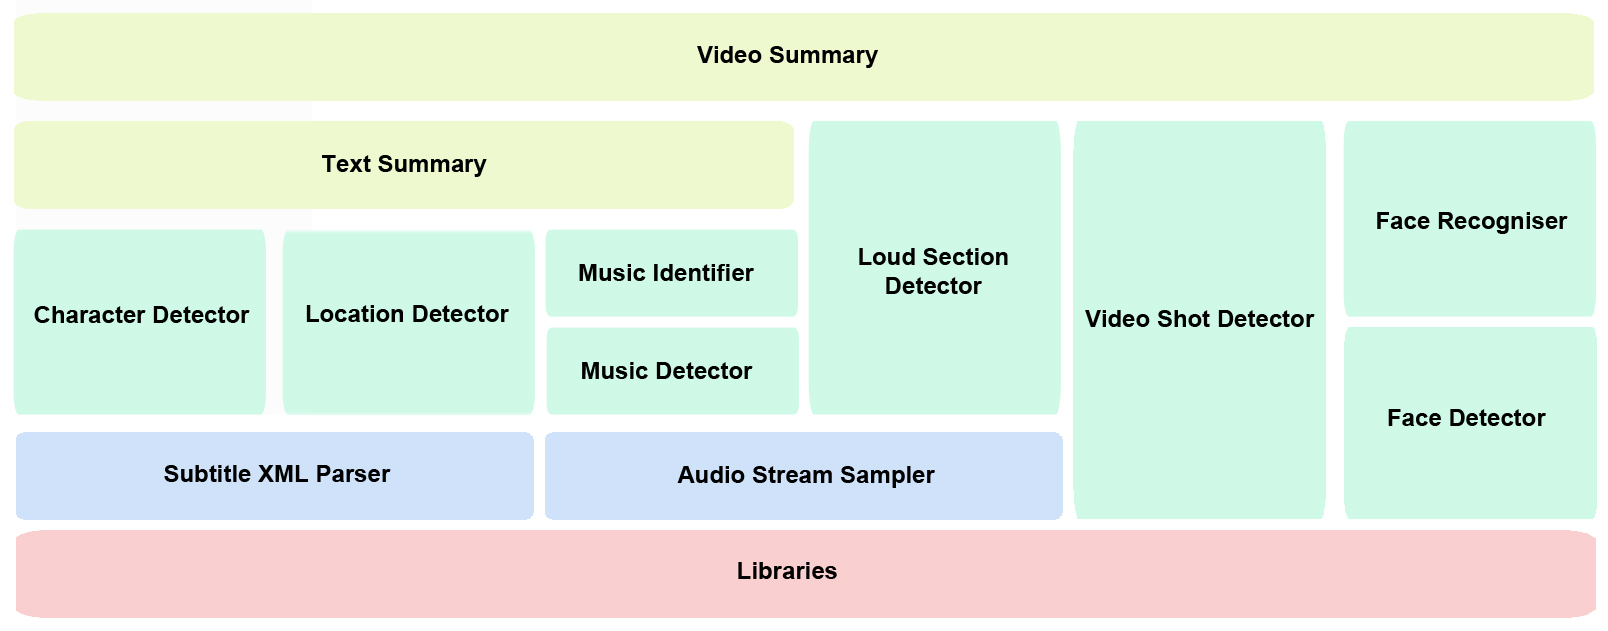
\includegraphics[trim = 0mm 0mm 0mm 0mm, clip, scale=0.27]{Images/design_overview_diagram.jpg}
\caption{Design Overview Diagram}
\label{fig:DesignOverview}
\end{figure}

\subsubsection{Text Based Analysis}
As detailed in the requirements (see Section \ref{sec:Requirements}) it is assumed that the system will have access to a DVB subtitle file for each video. This is in XML format so this will need to be processed by an XML parser. 

Natural Language Processing (NLP) can follow to assist in finding information which describes the video. This is likely to be faster from a computational perspective. Some interesting information to extract at this stage would be the main characters and the locations.

\subsubsection{Audio Analysis}
The next resource that the team can take advantage of is the audio track associated with each video. 
This will involve extracting and segmenting the audio stream, with a focus on the volume of each segment from the video which can be used to 
produce a list of the interesting timestamps. Assuming that for the most part a loud sequence in a video represents an exciting or 
interesting activity, the system will mark this as such and make it available for the summary stage.

In addition to this frequency analysis will be implemented for the purpose of discovering music segments in a video, which can then be 
identified. This is related to the IP Rights Assessment scenario in Section \ref{sec:ProjectProblem}.

\subsubsection{Facial Detection Analysis}
In order to identify the main characters of a video or set of videos face detection will be a necessary feature of our system. This will 
involve detecting the faces in the different frames of the video, clustering them together to differentiate between the different characters, 
and finally trying to identify the actors playing those characters. The facial detection and recognition module shall be implemented in the system, 
using the pre-existing OpenIMAJ features.

\subsubsection{Video Shot Segmentation}
Part of the analysis will involve splitting a video in appropriate places i.e. performing video processing to find shots in the video. This functionality is part of the OpenIMAJ library and so no algorithms need to be produced for this section. References to video shots will be held in memory and this information can then easily be used by other modules.

\subsubsection{Textual Summary}
The aim of the system will be to produce a textual summary of the interesting features of the videos. In addition the system will have the 
functionality to navigate to the interesting sections of the source video by using hyperlinks, which was suggested by the customer.The 
textual summary can contain information from each of the modules and can be combined together where applicable.

\subsubsection{Video Summary}
The goal of this module is for interesting sequences of video to be joined to produce a video summary of the original video to a target 
length, whilst still providing a good representation of its content. This will use the information gathered from the various modules to find interesting 
points in the video then using the video segmentation stage; the interesting shots can then be combined into sequences in order to create a smooth 
output video.

\newpage
\subsection{Design Patterns}

\subsubsection{Evaluation of Patterns}
The system essentially involves a user submitting a set of video data (either an episode, a series of episodes or a film) and selecting from 
a set of different options to generate a summary of that data. Due to its complicated nature various design patterns that involve 
simplifying the structure and the use of algorithms have been evaluated for their usefulness. 

\textbf{Model View Controller (MVC)}
\newline
\textbf{Description:} The MVC pattern involves splitting up the code so that the model deals with the data within the program, the View renders the 
display based on the data held in the Model and allows the user to interact with it whilst the Controller performs the actions specified by 
the user. The Controller has access to both the Model and the View and the View has access to the Model.
\newline
\textbf{Evaluation:} This pattern would be useful in structuring the code for this project as it contains a user interface that runs varying summarisation algorithms on the data submitted by the user so it fits perfectly into the pattern.

\textbf{Strategy Pattern}
\newline
\textbf{Description:} The strategy pattern involves defining a set of separate interchangeable algorithms that can be selected at runtime, 
independent of the user. 
\newline
\textbf{Evaluation:} This pattern would be very useful for the project as a number of different algorithms will be necessary to create the different summaries of the video content. The algorithms can be defined in different classes and can be selected at runtime depending on which summary options the user selects.

\textbf{Template Pattern}
\newline
\textbf{Description:} The template pattern involves outlining the skeleton of the main algorithm of the program with some of the steps being defined in subclasses so that the algorithm can run in different ways without changing its structure. 
\newline
\textbf{Evaluation:} This pattern could be appropriate for this project in the sense that every operation performed on the data will be a 
summarisation algorithm. However, given the range of different summaries that this project is looking to perform 
(main characters, main action sequence, potentially even music rights) it would be difficult and perhaps restricting to 
incorporate everything into one algorithm. 

\textbf{Composite Pattern}
\newline
\textbf{Description:} The composite pattern aims to ignore the difference between compositions of objects and individual objects. 
\newline
\textbf{Evaluation:} This pattern could be put to good use in this project, as generic algorithms could be defined to do either one scene of an episode,
a whole episode or even a collection of episodes.  

\textbf{Proxy Pattern}
\newline
\textbf{Description:} The proxy pattern provides an identical interface to the subject interface so that in certain instances a proxy can be substituted in place of the real subject.
\newline
\textbf{Evaluation:} This pattern could potentially be utilised in this project by creating a proxy for the video so that only the relevant parts could be loaded into the system with the rest being replaced by the proxy as suitable. 

\subsubsection{Proposed Solution}
The proposed solution is to combine the two most useful patterns, MVC and Strategy. The structure of MVC will be used to split up the code 
and the strategy pattern will be implemented in the Controller to separate the different summarisation algorithms needed to perform the 
operations specified in the View. This will keep with the theme of only showing the user the necessary components (the View) and will 
hide the Controller's actions (the different algorithms) from the user, as they should be independent from them. Other elements of the 
aforementioned patterns could also be added in as necessary, such as defining the strategy algorithms so that they could be ran on a 
composition of objects or an individual object (from the composite pattern). The functionality described by the proxy pattern could also be 
used when appropriate to provide a substituting interface dependent on the data entered into the system \cite{designRef}.

\subsubsection{Architecture Structure Diagram}
\begin{figure}[h1]
\begin{center}
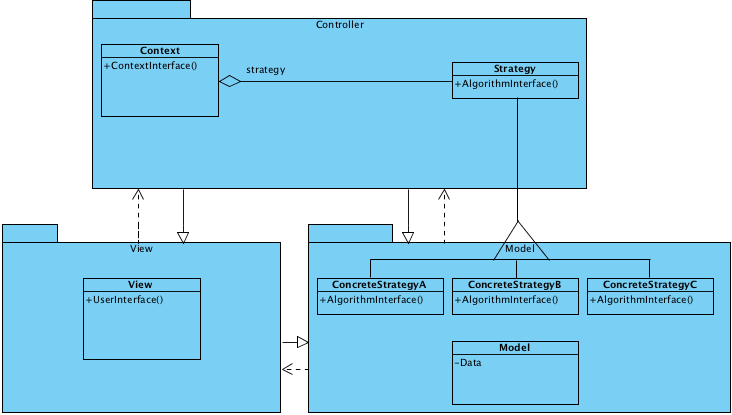
\includegraphics[trim = 0mm 0mm 0mm 0mm, clip, scale=0.61]{Images/StructureDiagram.png}
\end{center}
\caption{Design Overview Diagram}
\end{figure}

\newpage

\subsection{User Interface Design}
\label{sec:UIDesign}
The design of the team's user interface for the system is below:
\begin{figure}[h1]
\begin{center}
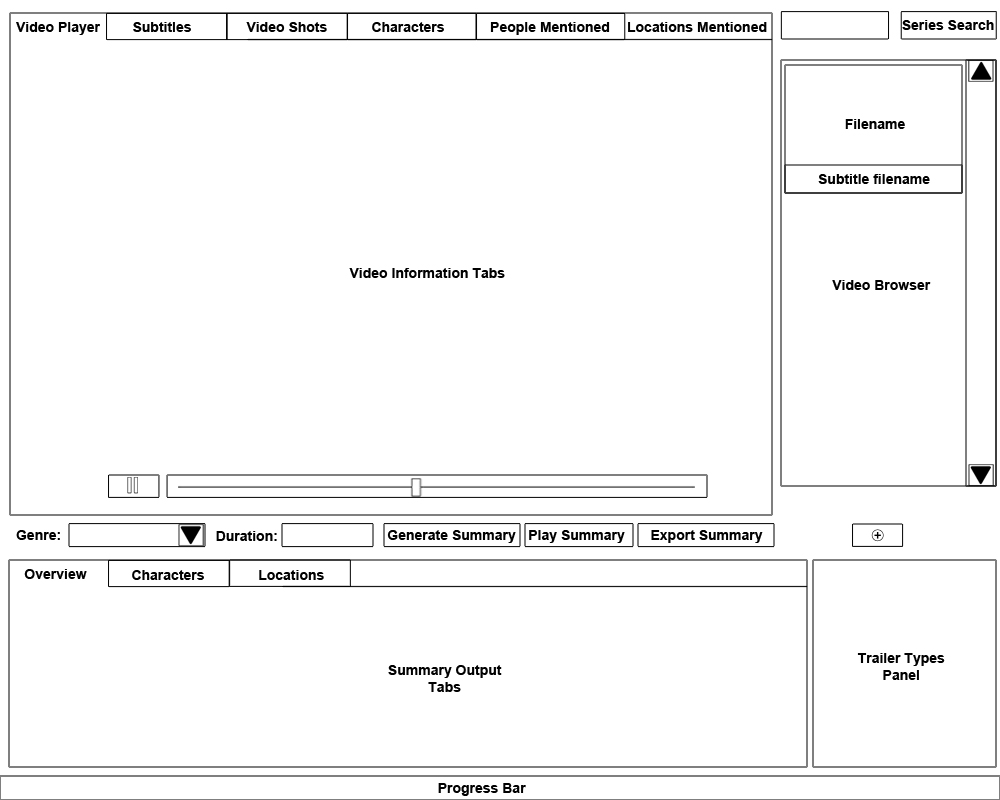
\includegraphics[trim = 0mm 0mm 0mm 0mm, clip, scale=0.43]{Images/user_interface_design.jpg}
\end{center}
\caption{User Interface Diagram}
\end{figure}

This has been designed in to enable users who have had previous experience with video editing programs to quickly get to grips with 
how to use the system effectively. Furthermore, by having a user interface it hides the complexity of the background processing, which also allows the video summarisation and the results it produces to be easily demonstrated to the team's supervisor, 
customer and anyone else who attends the presentations that are a part of the assesment criteria.

\newpage
\subsection{Prototype}
The prototyping stage had the main aim of getting the team to set up their development environments and ensure that they could work with the 
various tools and technologies that had been chosen in Section \ref{sec:ProjectTools}. For example, Maven \cite{citeMaven} is used to help 
with managing the building and deployment processes. Once Maven was set up on each development system and the project had been 
checked out from UGForge using SVN, it was straightforward to progress as a team. 

The first stage was to construct the basic Graphical User Interface (GUI) (the design of which is shown in Section \ref{sec:UIDesign}), 
followed by building the MVC packages and finally, producing skeleton classes for all backend modules as shown in 
Section \ref{sec:DesignOverview} in order to allow the structuring of the application correctly. Next, the ability to load video and subtitle 
files into the application was implemented. 

The modules were divided up amongst the individual team members in order that each individual could focus on a particular element or module of 
summarisation and were partially integrated into the GUI. The semi-complete features at the prototyping stage were shot detection, face 
detection and subtitle parsing, all of which produced output to the GUI at intermediate stages. This division allowed further understanding 
of the software libraries and also meant that a good demonstration of what was going on behind the scenes was available to show at Progress 
Seminar one.

The prototype provided a good foundation on which to start the implementation stage but also during the process, the team learnt about the 
OpenIMAJ software library and discovered a number
of bugs particularly concerning how efficiently the software would process the video. The team was in frequent contact with the developers 
of the software and were able to pass on any issues and receive feedback very quickly.
